\documentclass[oneside]{book}

\usepackage{amssymb}
\usepackage{graphicx}
\usepackage{eufrak}

\newtheorem{theorem}{Theorem}[chapter]
\newtheorem{lemma}[theorem]{Lemma}
\newtheorem{proposition}[theorem]{Proposition}
\newtheorem{corollary}[theorem]{Corollary}

\newenvironment{proof}[1][Proof]{\begin{trivlist}
\item[\hskip \labelsep {\bfseries #1}]}{\end{trivlist}}
\newenvironment{definition}[1][Definition]{\begin{trivlist}
\item[\hskip \labelsep {\bfseries #1}]}{\end{trivlist}}
\newenvironment{example}[1][Example]{\begin{trivlist}
\item[\hskip \labelsep {\bfseries #1}]}{\end{trivlist}}
\newenvironment{remark}[1][Remark]{\begin{trivlist}
\item[\hskip \labelsep {\bfseries #1}]}{\end{trivlist}}

\newcommand{\qed}{\nobreak \ifvmode \relax \else
      \ifdim\lastskip<1.5em \hskip-\lastskip
      \hskip1.5em plus0em minus0.5em \fi \nobreak
      \vrule height0.75em width0.5em depth0.25em\fi}

\begin{document}
\title{Notes and Solutions for ``Measure Theory and Integration" by Michael E. Taylor}
\author{Arya Pourzanjani} 
\date{\today}
\maketitle

%%%%%%%%%%%%%%%%
%%%%%%%%%%%%%%%%
\chapter{The Riemann Integral}
%%%%%%%%%%%%%%%%
%%%%%%%%%%%%%%%%

\section*{Solutions}
\begin{enumerate}
%%%%%%%%%
%%%%%%%%%
\item[7.] Since $f:[ac,bc]\to \mathbb{R}$ is Riemann integrable, by definition its integral is equal to its upper sum i.e.

\begin{eqnarray}
\label{eq:upperSumStretched}
\frac{1}{c}\int_{ac}^{bc} f(x)\,dx &=& \frac{1}{c} \inf_{\cal{P}} \bar{I}_{\cal{P}}(f) \nonumber \\
&=& \frac{1}{c} \inf_{\cal{P}} \sum_{k} \sup_{[x_k,x_{k+1}]} f(x)\, l([x_k,x_{k+1}])
\end{eqnarray}

Assume $c > 1$ for the sake of intuition here. They key insight to note here is that by multiplying the input of a function by a constant i.e. $f(cx)$ we effectively make it so that when going from left to right the function ``reaches" the numbers in its range earlier than it normally would and the function appears shrunken. Figure \ref{fig:sinSpedUp} shows an example.

\begin{figure}[h]
    \centering
    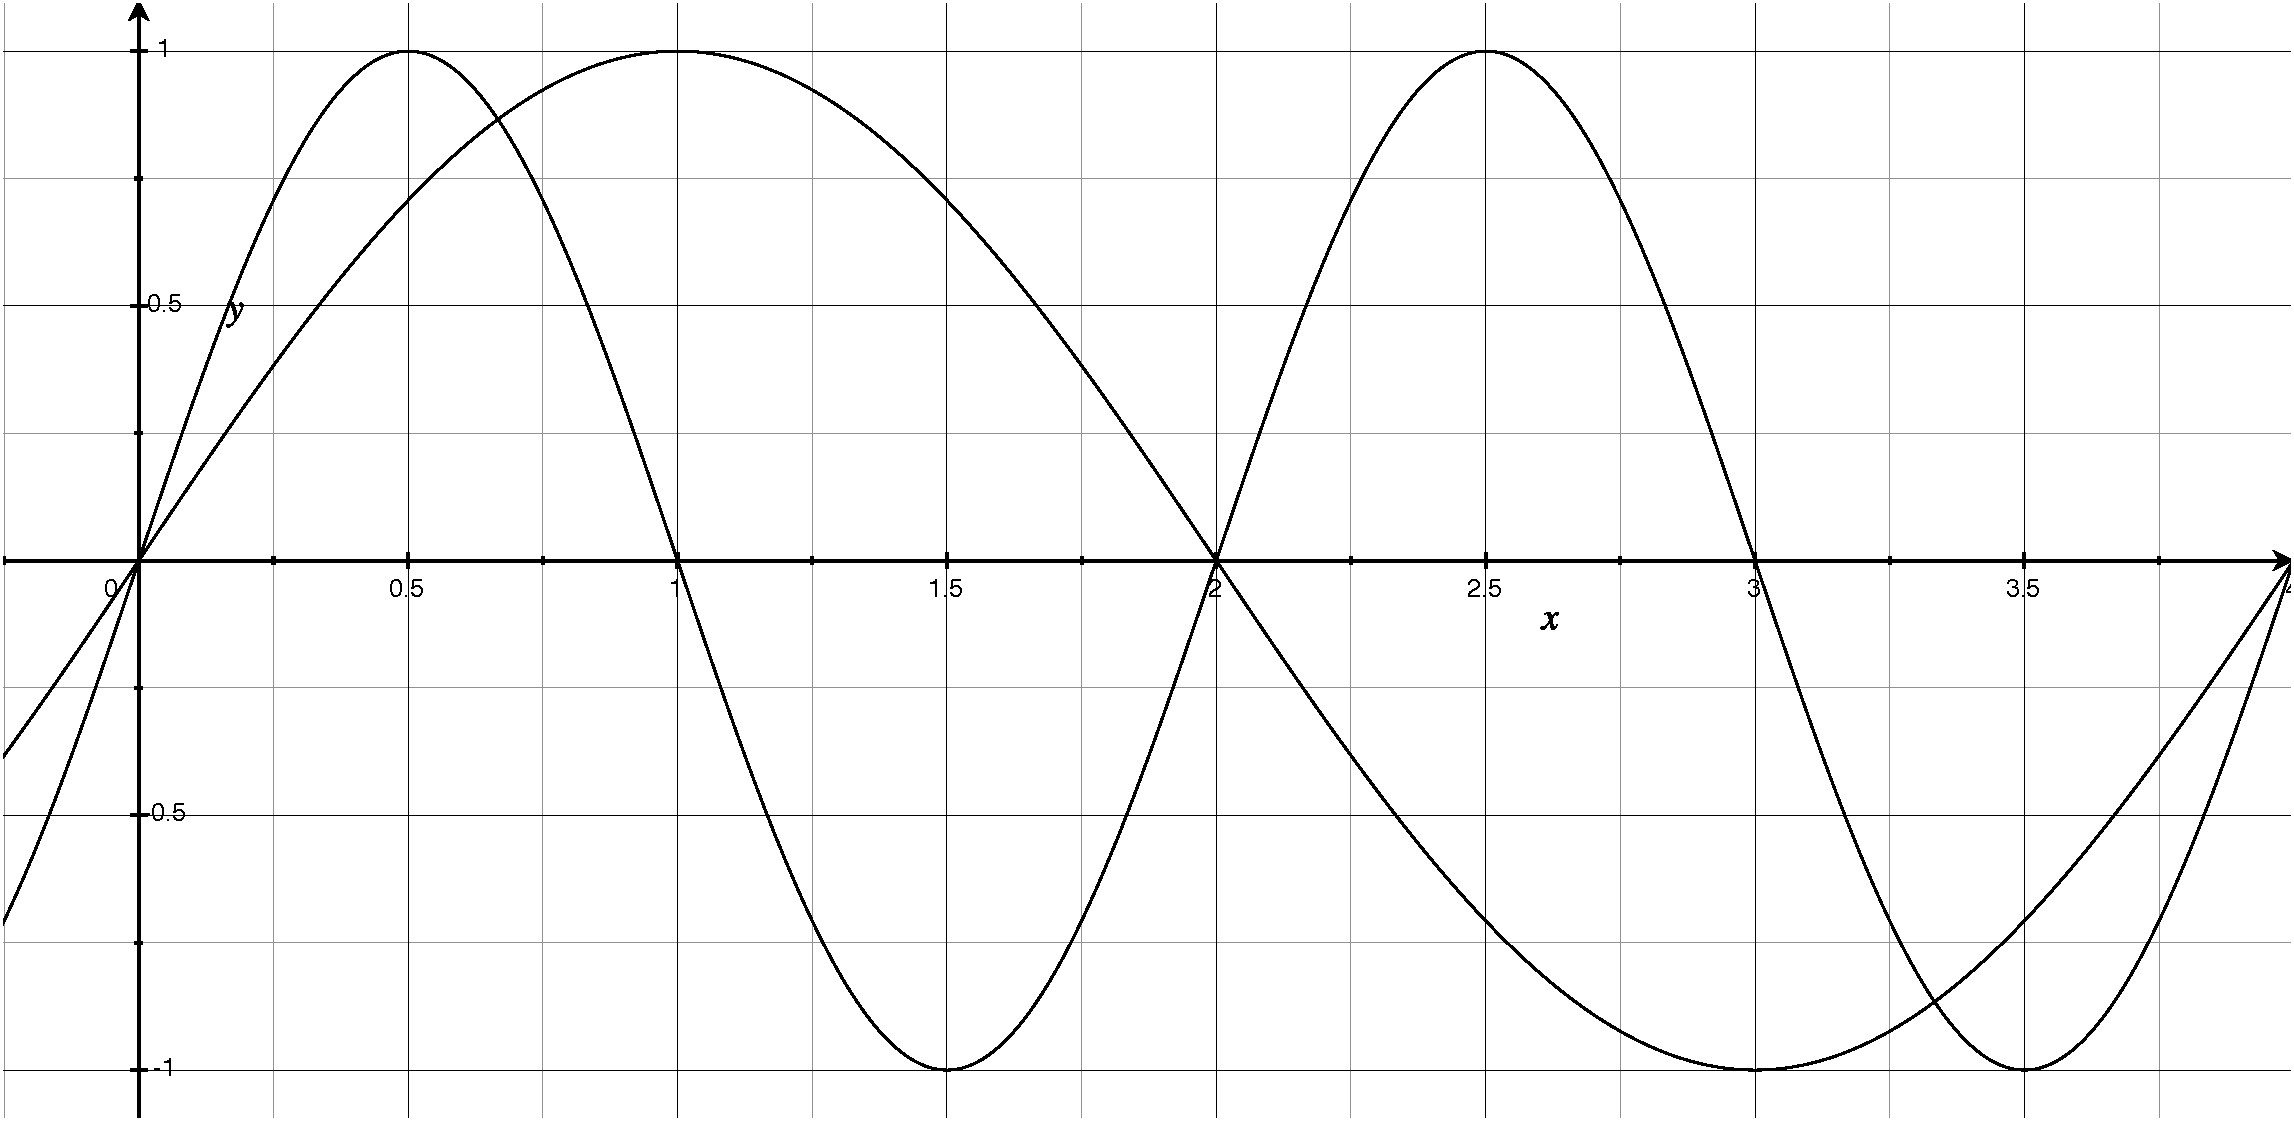
\includegraphics[width=0.6\textwidth]{sinSpeedUp.pdf}
    \caption{Graph of $\sin(\pi x/2)$ and it's ``sped up" or ``shrunken" counterpart $\sin(\pi x/2)$}
    \label{fig:sinSpedUp}
\end{figure}

Since $f(cx)$ reaches elements in its range earlier (and ``faster") than its stretched counterpart $f(x)$, the range of $f(x)$ over an interval $[x_k,x_{k+1}]$ is equivalent to the range of $f(cx)$ over the earlier and smaller interval $\left[\frac{x_k}{c},\frac{x_{k+1}}{c}\right]$. So equation \ref{eq:upperSumStretched} is equivalent to

\begin{eqnarray}
\label{eq:upperSumShrunk}
&& \frac{1}{c} \inf_{\cal{P}} \sum_{k} \sup_{\left[\frac{x_k}{c},\frac{x_{k+1}}{c}\right]} f(cx)\, l([x_k,x_{k+1}]) \nonumber \\
&=& \inf_{\cal{P}} \sum_{k} \sup_{\left[\frac{x_k}{c},\frac{x_{k+1}}{c}\right]} f(cx)\, l\left(\left[\frac{x_k}{c},\frac{x_{k+1}}{c}\right]\right)
\end{eqnarray}

The last equality comes from the fact that the length of $[x_k,x_{k+1}]$ is equal to the length of its shrunken counterpart multiplied by the shrink factor $c$. The shrink factor then cancelled out with the $1/c$ at the front of the expression.

Now it is clear though that equation \ref{eq:upperSumShrunk} is by definition $\bar{I}(f(cx))$. A parallel argument can be made for the lower sum and thus the equality is shown. Adding another term $d$ to the input make the function reach points in its range earlier, thus the function will be shifted to the left.

%%%%%%%%%
%%%%%%%%%
\item[8.] $f$ is continuous, which just means that if the two points \\$(x_1,s_1),(x_2,s_2) \in I \times S$ are less than a certain distance apart i.e. $d_{I \times S}((x_1,s_1),(x_2,s_2)) < \delta$ then $| f(x_1,s_1)-f(x_2,s_2) | < \omega(\delta)$. Now we need to show that $\varphi(y)$ has this same property, that is we need to show that if $d_S(s_1,s_2) < \delta$ then

\begin{eqnarray}
\label{eq:phiContinuous}
\left| \varphi(s_1) - \varphi(s_2) \right| &=& \left| \int_I f(x,s_1)\, dx - \int_I f(x,s_2)\, dx \right | < \omega(\delta)
\end{eqnarray}

Now we note that $d_{I \times S}((x,s_1),(x,s_2))=d_S(s_1,s_2)$ so if $d_S(s_1,s_2) < \delta$ then $d_{I \times S}((x,s_1),(x,s_2))< \delta$. Then from the continuity of $f$ this implies that $|f(x,s_1)-f(x,s_2)| < \omega(\delta)$, which in turn implies that

\begin{eqnarray}
&&\left| \int_I f(x,s_1)-f(x,s_2)\, dx \right | < l(I)\omega(\delta) \nonumber \\
&\Rightarrow& \left| \int_I f(x,s_1)\,dx- \int_I f(x,s_2)\, dx \right | < l(I)\omega(\delta) \nonumber \\
&\Rightarrow& \left| \varphi(s_1) - \varphi(s_2) \right| < l(I)\omega(\delta)
\end{eqnarray}

but this is exactly the property of continuity (equation \ref{eq:phiContinuous}) we wanted to show (up to a constant $l(I)$). The constant here is irrelevant because in words continuity means that the function can be as close as desired by making the inputs sufficiently close. The constant being there just means that we'd have to make the inputs a little closer to ensure the outputs are as close as we need them to be, but none the less we can ensure the outputs will be as arbitrarily close as need be.

%%%%%%%%%
%%%%%%%%%
\item[9.] Again we need to show that if  $d_S(s_1,s_2) < \delta$ then

\begin{eqnarray}
\label{eq:phi2Continuous}
&&\left| \varphi(s_1) - \varphi(s_2) \right| \nonumber\\
&=&\left| \int_{g_0(s_1)}^{g_1(s_1)} f(x,s_1)\, dx - \int_{g_0(s_2)}^{g_1(s_2)} f(x,s_2)\, dx \right |
\end{eqnarray}

Since $a \le g_0(y) < g_1(y) \le b$ these integrals are can be thought of as being evaluated over an interval that is to the right of $a$ by $\alpha_j := g_0(s_j)-a$ and smaller than $[a,b]$ by a factor of $\kappa_j :=l([g_0(s_j),g_1(s_j)])/l([a,b])$. From exercise 7 we know that we can stretch these functions and divide by the stretching factor to get an equivalent size interval. We can also translate the function the right to the left and still have an equivalent integral. By doing the latter first we see that \ref{eq:phi2Continuous} is equivalent to

\begin{eqnarray}
\left| \int_{a}^{g_1(s_1)-\alpha_1} f(x+\alpha_1,s_1)\, dx - \int_{a}^{g_1(s_2)-\alpha_2} f(x+\alpha_2,s_2)\, dx \right |
\end{eqnarray}

which by stretching is equivalent to

\begin{eqnarray}
\left| \frac{1}{\kappa_1} \int_{a}^{b} f\left(\frac{x+\alpha_1}{\kappa_1},s_1\right)\, dx - \frac{1}{\kappa_2} \int_{a}^{b} f\left(\frac{x+\alpha_2}{\kappa_2},s_2\right)\, dx \right|
\end{eqnarray}

and this is just the familiar condition \ref{eq:phiContinuous} from exercise 8 with a couple constant scalars that will not affect the limit.

%%%%%%%%%
%%%%%%%%%
\item[10.] This is another application of the idea from the last couple of problems: the idea that changing the input of a function makes the function reach its range faster or slower than it normally would. In this case, the ``speed" so to speak is a continuous function, so intuition would tell us that our stretch factor must also be continuous. By definition the integral is equal to its upper limit

\begin{eqnarray}
\label{eq:10start}
\int_{\varphi(a)}^{\varphi(b)} f(y)\,dy = \inf_{\cal{P}} \sum_k \sup_{[y_k,y_{k+1}]} f(y)\,l([y_k,y_{k+1}])
\end{eqnarray}

Now we must relate this quantity to a similar quantity that has its input transformed by $\varphi$. We look to an example in Figure \ref{fig:varPhiEx} for motivation.

\begin{figure}[h]
    \centering
    \includegraphics[width=0.6\textwidth]{Ch1_10.pdf}
    \caption{Example of a function $\varphi(x)$ that is differentiable and has continuous derivative on a neighborhood and positive derivative on the rest of $[a,b]$.}
    \label{fig:varPhiEx}
\end{figure}

The key point to note here is that $\varphi$ provides a continuous one-to-one map from $[x_k,x_{k+1}]$ to $[y_k,y_{k+1}]$ so the range of $f(y), y \in [y_k,y_{k+1}]$ is the exact same set as $f(\varphi(x)), x \in [x_k,x_{k+1}]$. Thus \ref{eq:10start} is equal to

\begin{eqnarray}
\label{eq:10_2}
\inf_{\cal{P}} \sum_k \sup_{[x_k,x_{k+1}]} f(\varphi(x))\,l([y_k,y_{k+1}])
\end{eqnarray}

Now note that $l([x_k,x_{k+1}]) = x_{k+1}-x_k$ and $l([y_k,y_{k+1}]) = y_{k+1}-y_k=\varphi(x_{k+1})-\varphi(x_k)$ so \ref{eq:10_2} is equal to

\begin{eqnarray}
\label{eq:10almost}
&&\inf_{\cal{P}} \sum_k \sup_{[x_k,x_{k+1}]} f(\varphi(x))\,l([y_k,y_{k+1}]) \frac{l([x_k,x_{k+1}])}{l([x_k,x_{k+1}]) } \nonumber \\
&=& \inf_{\cal{P}} \sum_k \sup_{[x_k,x_{k+1}]} f(\varphi(x))  \frac{\varphi(x_{k+1})-\varphi(x_k)}{x_{k+1}-x_k} \,l([x_k,x_{k+1}])
\end{eqnarray}

Taking smaller and smaller intervals will get \ref{eq:10almost} arbitrarily close to $\bar{I}(f(\varphi)\varphi')$ and a parallel argument can be made for the lower limit.

%%%%%%%%%
%%%%%%%%%
\item[11.] We first derive the product rule. By definition of the derivative

\begin{eqnarray}
\frac{d}{dx} (f(x) g(x)) = \lim_{h \to 0} \frac{1}{h} [f(x+h)g(x+h) - f(x)g(x)]
\end{eqnarray} 

Adding $f(x)g(x+h)-f(x)g(x+h)$ gives us

\begin{eqnarray}
&&\lim_{h \to 0} \frac{1}{h} [(f(x+h)-f(x))g(x+h) + f(x)(g(x+h)-g(x))] \nonumber \\
&=& \lim_{h \to 0} \frac{1}{h} [(f(x+h)-f(x))g(x+h)] + \lim_{h \to 0} \frac{1}{h} [f(x)(g(x+h)-g(x))] \nonumber \\
&=& f'(x)g(x) + g'(x)f(x)
\end{eqnarray} 

Thus 

\begin{equation}
\frac{d}{dx} (f(x) g(x)) = f'(x)g(x) + g'(x)f(x)
\end{equation}

And the integrals over the functions from $a$ to $b$ are also equal making the left side

\begin{equation}
[f(b)g(b)-f(a)g(a)]
\end{equation}

by the fundamental theorem of calculus and the right side equal to

\begin{equation}
\int_a^b f'(x)g(x)\, dx + \int_a^b g'(x)f(x)\,dx
\end{equation}

giving us the desired result.

%%%%%%%%%
%%%%%%%%%
\item[14.] We derive the fundamental theorem of calculus from first principles. Since $G'$ is Riemann integrable then by Corollary 1.4 when the max size of a sequence of partitions $\cal{P}$ goes to zero then

\begin{eqnarray}
\int_a^b G'(t)\,dt &=& \lim_{\nu \to \infty} \sum_{k=1}^\nu G'(\xi_{\nu k}) l(J_{\nu k})
\end{eqnarray}

where we take $\xi_{\nu k}$ to be the end point of every interval, $x_{\nu k}$. Now as $\nu \to \infty$ the end points of each interval $J_{\nu k}$ i.e. $x_{\nu k}$ and $x_{\nu k+1}$ get closer and closer so it is equivalent to write the derivative in terms of the limit of $\nu$.

\begin{eqnarray}
&&\lim_{\nu \to \infty} \sum_{k=1}^\nu \frac{G(x_{\nu x_{k+1}})-G(x_{\nu k})}{x_{\nu x_{k+1}}-x_{\nu x_{k}}} l(J_{\nu k}) \nonumber \\
&=& \lim_{\nu \to \infty} \sum_{k=1}^\nu G(x_{\nu x_{k+1}})-G(x_{\nu k}) \nonumber \\
&=& \lim_{\nu \to \infty} G(b) - G(a) \nonumber \\
&=& G(b) - G(a)
\end{eqnarray}

\end{enumerate}
%%%%%%%%%%%%%%%%
%%%%%%%%%%%%%%%%
\chapter{Lebesgue Measure on the Line}
%%%%%%%%%%%%%%%%
%%%%%%%%%%%%%%%%

There are many collections of open sets that can cover an interval $I$, these are called the covers of $I$. The covers of $I$ are themselves a set and each element in this set has a length. Thus these lengths can also be thought of a set. There is also a set of numbers that are less than or equal than all lengths in this set. The maximum of this set is the infimum of the lengths set and the outer measure of $I$.

There's always a cover of $I$ whose length is greater than the outer measure by some arbitrary length, otherwise it the outer measure wouldn't be the outer measure. 

\begin{lemma}[2.2]

\end{lemma}

\begin{proof}
We'd like to show that one can always find an open set that covers $K$ such that $m^*(\mathcal{O} \setminus K) \le \varepsilon$. We already know we can always find an open set that covers $K$ such that $m^*(\mathcal{O}) \le m^*(K) + \varepsilon$.
\end{proof}

\section{Super and Sub-Additivity}
Subadditivity means that if $S_1$ and $S_2$ are two subsets of $I$ then

\begin{equation}
\label{eq:subadditivity}
m^*(S_1 \cup S_2) \le m^*(S_1) + m^*(S_2).
\end{equation}

In words this is saying that the infimum length of all open covers of $S_1 \cup S_2$ is smaller than the sum of the infimum lengths of open covers of $S_1$ and $S_2$. There are three collections of sets in play here. There are the collections of open covers of $S_1$ and $S_2$ which we call $\{\mathcal{O}_1\}$ and $\{\mathcal{O}_2\}$ respectively and there are the collections of open covers of $S_1 \cup S_2$ which we'll call $\{\mathcal{O}_\cup\}$. Remember again these are collections of sets. There are several possible open covers. 

The key observation to make is that any if you pick any single cover from the collection $\{\mathcal{O}_1\}$, call it simply $\mathcal{O}_1$ and any cover from the collection $\{\mathcal{O}_2\}$, called $\mathcal{O}_2$ then their union $\mathcal{O}_1 \cup \mathcal{O}_2$ is also a cover of $S_1 \cup S_2$ and hence a member of the collection of open covers $\{\mathcal{O}_\cup\}$. So $\{\mathcal{O}_\cup\}$ contains all open covers of the form $\mathcal{O}_1 \cup \mathcal{O}_2$ and then some! $\{\mathcal{O}_\cup\}$ could also include covers that have smaller length than those of the form $\mathcal{O}_1 \cup \mathcal{O}_2$, which is the intuition behind the inequality \ref{eq:subadditivity}.

A similar logic can be used for inner-measures. Inner measures are defined as 

\begin{equation}
\label{eq:innerMeasure}
m_*(S) = m^*(I) - m^*(I \setminus S) = l(I) - m^*(I \setminus S)
\end{equation}

By definition we have that

\begin{eqnarray}
m_*(S_1) + m_*(S_2) = l(I)-m^*(I \setminus S_1) + l(I)-m^*(I \setminus S_2)
\end{eqnarray}

Now we are concerned with the collection of open covers of $I \setminus S_1$ and $I \setminus S_2$ respectively. Observe that the collection of open covers of $I \setminus (S_1 \cup S_2)$ is a subset of the collection of open covers that are the unions of open covers of $I \setminus S_1$ and $I \setminus S_2$.

\section*{Solutions}
\begin{enumerate}
%%%%%%%%%
%%%%%%%%%
\item[2.] Each of the $S_j$ are measurable so the difference of two consecutive $S_j$ when $j \ge 2$, i.e. $T_j :=S_j \setminus S_{j-1}$ is measurable. Now if we define $T_1 := S_1$ then 

\begin{eqnarray}
m(S_j) = m \left( \bigcup_{l = 1}^j T_j \right) = \sum_{l=1}^j m(T_j)
\end{eqnarray}

Since a measure is always greater than or equal to zero then this sum is increasing as $j$ increases, and we can always find a $j$ such that the sum is within $\epsilon > 0$ of the infinite sum $\sum_{l \ge 1} m(T_j)$ hence we write

\begin{eqnarray}
\sum_{l=1}^j m(T_j) \nearrow \sum_{l \ge 1} m(T_j)
\end{eqnarray}

But again the $T_j$ are disjoint so we have

\begin{eqnarray}
\sum_{l \ge 1} m(T_j) = m\left( \bigcup_{l \ge 1} T_j \right)  = m(S)
\end{eqnarray}

%%%%%%%%%
%%%%%%%%%
\item[3.] Since each of the $S_j$ are measurable the intersection of a finite number of them is measurable. Furthermore, the measure of the complement of a measurable set is the length of the interval minus the measure of the set so putting these together we have

\begin{eqnarray}
\label{eq:measDec}
m(S_j) = m \left( \bigcap_{l=1}^j S_j \right) = m \left( I \setminus \left[ \bigcup_{l=1}^j (I \setminus S_j) \right] \right) = l(I)- m \left(  \bigcup_{l=1}^j (I \setminus S_j)  \right)
\end{eqnarray}

We now rewrite this union as the union of disjoint sets by defining $R_1 := I \setminus S_1$

\begin{equation}
\label{eq:Rdef}
R_j := (I \setminus S_j) \setminus \left[ \bigcup_{l=1}^{j-1} (I \setminus S_l) \right]
\end{equation}

In words, each $R_j$ includes only the new elements $I \setminus S_j$ added to $\bigcup_{l=1}^{j-1} (I \setminus S_l)$ that the former didn't already have. thus we can rewrite \ref{eq:measDec} as

\begin{equation}
l(I) - m\left( \bigcup_{l=1}^j R_l \right)
\end{equation}

or since the $R_l$ are all disjoint

\begin{equation}
l(I) - \sum_{l=1}^j m\left(  R_l \right)
\end{equation}

Since measure are always greater than or equal to zero, this value decreases as $j$ increases because we're always subtracting from $l(I)$ an additional number, but it doesn't go below zero. This is because $\bigcup_{l \ge 1} R_l = S \subset I$. In fact 

\begin{equation}
\sum_{l=1}^j m\left(  R_l \right) \nearrow \sum_{l \ge1} m\left(  R_l \right) = m \left(\bigcup_{l \ge 1} R_l \right) = m \left(\bigcup_{l \ge 1} (I \setminus S_l) \right)
\end{equation}

%%%%%%%%%
%%%%%%%%%
\item[4.]  We are no longer dealing with an interval but the countable union of intervals that intersect at most one point and make up the real line i.e. $\bigcup_k I_k$. On the real line the measure of a set $S$ is define as the sum of measures of $S$ intersected with each of the intervals $I_k$ that make up $\mathbb{R}$, that is $m(S)=\sum_k m(S \cap I_k)$. The same logic for exercise 2 works for the countable union case since we did not say anything about the measure of the whole metric space. As far the countable intersection case since we still have that $S_j = \bigcap_{l=1}^j S_l$ so every time we intersect $\bigcap_{l=1}^{j-1}$ with $S_j$ we can think of the resulting set as $\bigcap_{l=1}^{j-1}$, as the running intersection with some elements taken away. Another perspective is that we are keeping a running union of the complement $\bigcup_{l=1}^{j-1} (\mathbb{R} \setminus S_l)$ and we are adding a bit each time we union it with $\mathbb{R} \setminus S_j$ to get the resulting $\bigcup_{l=1}^{j} (\mathbb{R} \setminus S_l)=\mathbb{R} \setminus S_j$. Now define $R_1 := \mathbb{R} \setminus S_1$ and define

\begin{equation}
R_j := (\mathbb{R} \setminus S_j) \setminus \left[ \bigcup_{l=1}^{j-1} (\mathbb{R} \setminus S_l) \right]
\end{equation}

to be this bit we are adding every time. Let us write the following

\begin{eqnarray}
m(S_j) &=& m(\mathbb{R} \setminus (\mathbb{R} \setminus S_j)) \nonumber\\
&=& m \left( \mathbb{R} \setminus \left[ \bigcup_{l=1}^{j} (\mathbb{R} \setminus S_l) \right] \right)\nonumber\\
&=& m\left(\mathbb{R} \setminus \bigcup_{l=1}^{j} R_l \right)
\end{eqnarray}

or by definition of measures on $\mathbb{R}$

\begin{eqnarray}
&=& \sum_k m\left(\left[ \mathbb{R} \setminus \bigcup_{l=1}^{j} R_l \right] \cap I_k \right) \nonumber \\
&=& \sum_k m\left( I_k \setminus \bigcup_{l=1}^{j} R_l  \right)\nonumber \\
&=& \sum_k \left\{ m( I_k)-m\left( \bigcup_{l=1}^{j} (R_l \cap I_k)  \right) \right\} \nonumber \\
&=& \sum_k \left\{ m( I_k)- \sum_{l=1}^j m(R_l \cap I_k)\right\}
\end{eqnarray}

 and since the $R_l$ are disjoint
 
\begin{eqnarray}
\label{eq:measureSj}
&=& \sum_k m(\mathbb{R}) - \sum_{l=0}^j m\left( R_l \right)
\end{eqnarray}
 
Notice that the union of the $R_j$ up to $j$ is $\bigcup_{l=1}^j (\mathbb{R} \setminus S_l)=(\mathbb{R} \setminus S_j)$, the $R_j$ are disjoint from each other, and they are all measurable. Since they are measurable their measure is

\begin{equation}
m(R_j) = \sum_k m(R_j \cap I_k)
\end{equation}

so let us rewrite equation \ref{eq:measureSj} as
 
\begin{eqnarray}
&=& \sum_k m(I_k) - \sum_{l=0}^j \sum_k m(R_l \cap I_k) \nonumber\\
&=& \sum_k m(I_k) - \sum_k \sum_{l=0}^j m(R_l \cap I_k) \nonumber\\
&=& \sum_k \left\{ m(I_k) -\sum_{l=0}^j  m(R_j \cap I_k) \right\}
\end{eqnarray}

Remember each $R_j$ was adding a few elements to our running union now we are just thinking about it as the elements it adds to each $I_k$. If $R_j$ adds elements that have finite measure then $\sum_k m(R_j \cap I_k)$ is finite and in that case we can switch the sums to get

\begin{eqnarray}
&=& \sum_k m(I_k) -\sum_k \sum_{l=0}^j  m(R_j \cap I_k)\nonumber \\
&=&  \sum_k \left\{ m(I_k) -\sum_{l=0}^j  m(R_j \cap I_k) \right\}
\end{eqnarray}



%%%%%%%%%
%%%%%%%%%
\item[5.] We want to prove that if a countable collection of sets $\{S_j\}$ are in a family $\mathfrak{F}$ that their intersection is as well i.e. that $\bigcap_{j \ge 1} S_j \in \mathfrak{F}$. Note that

\begin{eqnarray}
\bigcap_{j \ge 1} S_j &=& X \setminus \left( \bigcup_{j \ge 1} (X \setminus S_j) \right)
\end{eqnarray}

Each of $(X \setminus S_j)$ are in $\mathfrak{F}$ because they are complements of members of $\mathfrak{F}$. Thus the countable union and in turn its complement are all in $\mathfrak{F}$.

%%%%%%%%%
%%%%%%%%%
\item[6.] Define $S_{\cup} := \bigcup_{j \ge 1} S_j$ then

\begin{eqnarray}
\bigcap_{j \ge 1} S_j = S \setminus \left( \bigcup_{j \ge 1} (S \setminus S_j) \right)
\end{eqnarray}

%%%%%%%%%
%%%%%%%%%
\item[7.] For any rational number $q_1$ there is always a rational number $q_2$ we can add to it to get any third rational number $q_3$ that we desire. What about irrational numbers? Can we had a rational number to $q_1$ and get $q_3 = \pi$? No, because $\pi$ is irrational and so there's no two rational numbers we can add that equal it. If $q_1=\pi-1/2$ we could add the rational number $1/2$ to get $q=\pi$. So by adding rational numbers to $\pi$ we can reach some irrational numbers, but we can't reach rational ones. Note we can't reach all irrational numbers, e.g. there is no rational number you can add to $\pi$ to get $\sqrt{2}$. So the rational numbers, $\pi$, $\sqrt{2}$, etc. all have associated families of numbers you can reach by adding a rational number to them. These families are called orbits and there an uncountable number of them.

If we take one element from every orbit and call this set $S$. Then we can use the elements of $S$ as a basis in the sense that we can create any number in $\mathbb{R}$ by taking one of our basis numbers and adding a rational numbers. Say from the $\pi$ orbit we choose $\pi$, then we can create $3.26459...=\pi+3.23$ by simply adding $3.23$ to $\pi$.  

Now let $S_\alpha$ be $S$ all the elements of $S$ shifted by $\alpha$, so if $\pi \in S$ then $\pi+\alpha \in S_\alpha$. Now lets examine the countable union $\bigcup_{\alpha \in \mathbb{Q}} S_\alpha$. By construction this union equals the real line. On the other hand each $S_\alpha$ is disjoint from every other $S_\alpha$ also by construction but they all have the same measure.

Since $X$ has positive measure there must be some $I_k$ where $m(X \cap I_k) > 0$. Let us examine its measure

\begin{eqnarray}
0<m^*(X \cap I_k) = m^*(X \cap I_k \cap \mathbb{R}) 
\end{eqnarray}

Keep in mind since the union of all $S_\alpha$ is $\mathbb{R}$ we have

\begin{eqnarray}
= m^*(X \cap I_k \bigcup_{\alpha \in \mathbb{Q}} S_\alpha) = m^*\left(\bigcup_{\alpha \in \mathbb{Q}} (X \cap I_k \cap S_\alpha)\right)
\end{eqnarray}

By subadditivity

\begin{eqnarray}
\le \sum_{\alpha \in \mathbb{Q}}m^* (X \cap I_k \cap S_\alpha)
\end{eqnarray}

but since the $S_\alpha$ all have equal measure. Now we have that 

\begin{eqnarray}
\infty > m(I_k) \ge m_*(X \cap I_k) = m_*\left(\bigcup_{\alpha \in \mathbb{Q}} (X \cap I_k \cap S_\alpha)\right)
\end{eqnarray}

by superadditivity

\begin{eqnarray}
\ge \sum_{\alpha \in \mathbb{Q}}m_* (X \cap I_k \cap S_\alpha)
\end{eqnarray}

but all the measure of the terms in the sum are equal because the $S_\alpha$ all 

%%%%%%%%%
%%%%%%%%%
\item[8.] Figure \ref{fig:cantorSets} depicts the first few of these sets. 

\begin{figure}[h]
    \centering
    \includegraphics[width=0.8\textwidth]{cantorSets.png}
    \caption{First four Cantor Sets}
    \label{fig:cantorSets}
\end{figure}

There measure of the first few sets is $m(K_0)=1$,$m(K_1)=2/3$,$m(K_2)=4/9$. In general we have

\begin{equation}
m(K_\nu) = \left( \frac{2}{3} \right)^{\nu}
\end{equation}

From exercise 3, we know that if $K_\nu$ is a decreasing sequence of measurable subsets the measure of their limit is the limit of their measure i.e. $m(K_\nu) \searrow m(K)$ so 

\begin{equation}
m(K) = \lim_{\nu \to \infty} m(K_\nu) = \lim_{\nu \to \infty} \left( \frac{2}{3} \right)^{\nu} = 0
\end{equation}

%%%%%%%%%
%%%%%%%%%
\item[9.] Figure \ref{fig:cantorSets2} depicts the first few of these sets.

\begin{figure}[h]
    \centering
    \includegraphics[width=0.8\textwidth]{cantorSets2.png}
    \caption{First four sets $L$}
    \label{fig:cantorSets2}
\end{figure}

Each turn we are subtracting $2^{\nu-1}$ sets of size $(1/5)^\nu$

\begin{equation}
m(L) = \lim_{\nu \to \infty} m(L_\nu) = \lim_{\nu \to \infty} 1 - \sum_{n=1}^\nu 2^{n-1} \left( \frac{1}{5} \right)^{n} = \lim_{\nu \to \infty} 1 - \frac{1}{2} \sum_{n=1}^\nu \left( \frac{2}{5}^n \right)
\end{equation}

Which is equal to $1/3$.

%%%%%%%%%
%%%%%%%%%
\item[10.] In ternary, once we remove the middle third what remains is all elements of the reals from 0 to $0.1$ and all the elements from $0.2$ to 1. But note that $0.1$ is equivalent to $0.022222\cdots$. In other words, what remains after we remove the middle third is all numbers that have a ternary representation with no 1's. If we remove the middle ninth of the first interval, we get all numbers from $0$ to $0.01=0.022222\cdots$. Going on in this way we can imagine $K$ as all ternary numbers between 0 and 1 that have a representation without ones. 

If we remove the middle fifth of the unit interval we get (in quinary) all numbers between 0 and $0.2=0.1444\cdots$ and all numbers between $0.3$ and 1. So we can say that what is left is all numbers with a quinary representation that doesn't include a 2 in the first digit after the decimal. Similarly if the we remove the middle fifth from the interval $[0,0.2]_5$ we get all numbers between $0.02=0.01444\cdots$ and $0.03$. Thus the Cantor middle fifth set consists of all numbers on the unit interval that have a quinary representation with no 2's in it.

Now let us recall the set $S$ that consists of one element from each orbit of $(0,1)$ by adding rational numbers. Recall that $S$ was not measurable i.e. $m^*(S) \neq m_*(S)$. Also recall that $L$ has positive measure it includes unmeasurable portion we'll call $S_L$. Now $f(S_L)$ is a subset of $K$ therefore it's outer measure must be less than the outer measure of $K$, but the outer measure of $K$ is just zero so the outer measure of $f(S_L)$ must be zero and its greater than its inner-measure so it's inner-measure must also be zero, therefore $f(S_L)$ is a Lebesque measurable but it's pre-image is not. 

\end{enumerate}
%%%%%%%%%%%%%%%%
%%%%%%%%%%%%%%%%
\chapter{Integration on Measure Spaces}
%%%%%%%%%%%%%%%%
%%%%%%%%%%%%%%%%

A function $f(x)$ is measurable if for every open interval $J \in \mathbb{R}$ we have that $f^{-1}(J) \subset \mathfrak{F}$. Take a look at the example function $f:\mathbb{R} \to \mathbb{R}$ in Figure \ref{fig:borelFunction.}. Here let's define our measure space $\mathfrak{F}$ to be the Borel sets. 

\begin{figure}[h]
    \centering
    %\includegraphics[width=1.0\textwidth]{borelFunction.png}
    \caption{Pre-images of a decreasing sequence of open sets.}
    \label{fig:borelFunction}
\end{figure}

This function is $\mathfrak{F}$ measurable so the preimage of any open set is in $\mathfrak{F}$ i.e. it is one of the Borel sets. What about closed intervals, say for example the interval $[1.5,2]$, is the preimage of that interval in $\mathfrak{F}$? Well $(0.5,3)$ is open so its pre-image, we'll call it $(x_{a1},x_{b1}) \in \mathfrak{F}$. The interval $(1,2.5)$ is also open so its pre-image $(x_{a2},x_{b2}) \in \mathfrak{F}$. In general, the sets $(1.5-1/n,2+1/n),\, n=1,2,\cdots$ are all open so their pre-images $(x_{an},x_{bn})$ are all members of $\mathfrak{F}$.

Remember  in a measure space we always choose $\mathfrak{F}$ to be closed under countable intersections, countable unions, and complements. Thus $\bigcap_{n =1}^n(x_{an},x_{bn}) \in \mathfrak{F}$, but this intersection turns out to be the close interval $[x_a,x_b]$ which has the closed image $[1.5,2]$. So since the pre-image of the closed interval $[1.5,2]$ is indeed in $\mathfrak{F}$. 

In general, the pre-image of any borel set in $\mathbb{R}$ will always be Borel in $X$, thus we can construct it by using the open sets in $X$, which are of course pre-images of open sets in $\mathbb{R}$.

\section{Open Sets and Borel Sets}
If you have a set $S \subset \mathbb{R}$ its pre-image is the set of all $x \in X$ such that $f$ maps $x$ to an element in $S$. Now let's imagine all the subsets of $\mathbb{R}$ that have pre-images in the $\sigma$-algebra $\mathfrak{F}$, let's call this collection $\mathfrak{S}$. Let $S := \bigcup_{j \ge 1} S_j$ be the countable union of sets in $\mathfrak{S}$.  The pre-image of this set is the set of elements in $X$ that $f$ maps to it, but if an $f$ maps an element  $x \in X$ to an element  $s \in S$ it's because at least one of the constituent sets $S_j$ that make up $S$ contained that same $s$, but if that's the case the pre-image of $S_j$ will include $x$. Thus we can see that $f^{-1}(\bigcup_{j \ge 1} S_j) = \bigcup_{j \ge 1} f^{-1}(S_j) \in \mathfrak{F}$.

Similarly, for any $S \in \mathfrak{S}$ since the pre-image of $S$ is in $\mathfrak{F}$ then the complement of the pre-image $X \setminus f^{-1}(S)$ is also in $\mathfrak{F}$, but these are all the elements in $X$ that $f$ does NOT map in to $S$ which is the pre-image of $\mathbb{R} \setminus S$. 

\section{Proposition 3.2} If one of the functions $f_j$ maps an element $x$ in to the point $s \in (a,\infty]$, then $g_1$ will map $x$ to a point $s^* \ge s$ thus $s^*$ will certainly be in $(a,\infty$ and thus $x$ will be included in $g_1's$ pre-image of $(a,\infty]$.

\section{Simple Functions}
If $S_j$ are in the $\sigma$-algebra $\mathfrak{F}$ then their characteristic functions are measurable because the pre-image of any open set will be $S_j$ if the open set contains one, or it will be in $X \setminus S_j$ if the open set does not contain one. Either way, both of these are in $\mathfrak{F}$ so the pre-image of any open set is in $\mathfrak{F}$ and that's what it means for a function to be measurable. We can also define the simple functions

\begin{equation}
\label{eq:simpleFunction}
\varphi(x)=\sum_{j=1}^N a_j \chi_{S_j}(x),\; a_j \in \mathbb{R}
\end{equation}

Note that an element $x \in X$ can be in one of the $S_j$'s or some of them or none of them. It can either be in or out of each $S_j$ so there are $2^N$ possibilities for which $S_j$ a single $x$ can show up in. Thus if $x$ is just in $S_j$ then $\varphi$ will map $x$ to $a_j$. If it's in $S_j$ and $S_j$ for example then $\varphi$ will map $x$ to $a_j+a_i$. $\varphi$ will map $x$ to the sum of $a_j$'s for whatever $S_j$ it shows up in. 

These are also measurable. There are only $2^N$ points in the image at most so open sets will contain none of them, some of them or all of them. To get the pre-image of an open set just find out which of these $2^N$ points it contains. The pre-image will be union of the pre-image of all these points. It's easy to get the pre-image of one of these points. The point is the sum of some combination of the $a_j$'s e.g. $a_1+a_5+a_6$. The points that $\varphi$ will map to this value are the points $x \in X$ that show up in all three of the sets (1)$S_1,S_5,S_6$ and (2)no other sets. The point that show up in these three sets is the intersection of the three which is in $\mathfrak{F}$ since its constituents are. The points $x$ that show up in no other sets are the points that are in the compliment of the union of all the sets. This is also in $\mathfrak{F}$. Thus the points we're concerned with are the points in both of these i.e. the intersection.

Since there are only $2^N$ possibilities of values each $x$ will take on we can rewrite \ref{eq:simpleFunction} so that it is the sum of $2^N$ terms each with their own coefficient we'll call $\tilde{a}_\sigma$ and simple function of the set that $\varphi$ maps to that coefficient. We'll call that set $\tilde{S}_\sigma$. 

\section{Lemma 3.3}
\begin{lemma}
If $\varphi \in \mathfrak{G}^+(X)$, then

\begin{equation}
\lambda(A) = \int_A \varphi\, d\mu = \int \chi_A \,\varphi\, d\mu
\end{equation}

is a measure on $\mathfrak{F}$
\end{lemma}

\begin{proof}
Recall that a measure is a function $\mu: \mathfrak{F} \to [0,\infty]$ that gives the empty set measure zero, and has the countable additivity property for disjoint sets. Recall that $\varphi(x)=\sum_{j=1}^N a_j \chi_{S_j}(x)$. We can think of $\chi_A$ as a filter of $\varphi$ because it either multiples by one, effectively doing nothing, or it multiplies by zero, ``filtering out" a value of $\varphi$. The values it doesn't filter out are those that are in $A$. Thus we have

\begin{equation}
\chi_A \varphi = \sum_{j=1}^N a_j \chi_{S_j \cap A}
\end{equation}
 
and

\begin{equation}
\int \chi_A \varphi\, d\mu = \sum_{j=1}^N a_j \mu(S_j \cap A)
\end{equation}
 
This quantity is definitely greater than or equal to zero since $\varphi \in \mathfrak{G}^+$. It definitely is zero when $A$ is the empty set. Now if $A$ is the countable disjoint union $\bigcup_{j \ge 1} A_j$ then

\begin{eqnarray}
\lambda \left( \bigcup_{j \ge 1} A_j \right) &=& \sum_{j=1}^N a_j \mu \left( S_j \cap \bigcup_{j \ge 1} A_j  \right) \nonumber \\
&=& \sum_{j=1}^N a_j \mu \left( \bigcup_{j \ge 1} (S_j \cap A_j)  \right) \nonumber \\
&=& \sum_{j=1}^N a_j \sum_{j \ge 1} \mu (S_j \cap A_j) \nonumber \\
&=&  \sum_{j \ge 1} \sum_{j=1}^N a_j \mu (S_j \cap A_j) \nonumber \\
&=&  \sum_{j \ge 1} \lambda(A_j)
\end{eqnarray}
 
\end{proof}

\section{Monotone Convergence Theorem}
Remember that the measurable functions $\mathcal{M}^+$ are the set of functions from $X$ to $[0,\infty]$ such that the pre-image of any open set is a set in the $\sigma$-algebra of $X$ we are concerned with, $\mathfrak{F}$. We can have an increasing sequence of such functions which just means if you look at one slice $f_j(x)$ for a single $x$ and increase $j$ this itself is a sequence. When we say $f_j \nearrow$ then that means we have a bunch of sequences (one for each $x \in X$) that are all increasing. We know these will all converge to a measurable function $f$, and since it's measurable it'll have an integral but the Monotone Convergence Theorem says the following will hold

\begin{theorem}{Monotone Convergence}
\begin{equation}
\int f\, d\mu = \lim_{n \to \infty} \int f_n\, d\mu
\end{equation}
\end{theorem}

So let's examine $\int f_n\, d\mu$. Since $f_n$ is always greater than or equal to all functions that came before it, we know that the pre-image of every set $(a,\infty]$ is pre-image of $(a,\infty]$ with respect to $f_n$, because if an earlier function was able to map an $x$ up there then $f_n$ was able to also. One can see that this pre-image is strictly increasing as $n$ increases, thus the measure of the pre-image is $\mu(f_j^{-1}((a,\infty])) \nearrow \mu(f^{-1}(a,\infty])$.

Now in terms of simple functions less than $f_n$ and simple functions less than $n$, we know that there's a finite number of ``levels" $a_j$ that will be hit so we can think of these integrals as the levels multiplied by the measure of the $x$ that got mapped to that level, but for a given level as we just saw $f_n$ will always have mapped $x$ with a measure that's less than or equal to what $f$ has mapped. As $n$ increase however, the measures for each level will begin to get converge to the measure $f$ assigns. Thus the levels stay the same and the measures at those levels converge to the $f$ levels so the then the integrals of the simple functions match. The integrals of the measurable functions are the supremums of their respective simple functions though so we have the theorem.

\section{Fatou's Lemma}

\subsection{liminf and limsup}
Remember that for a single $x$, $f_{j}(x),\, j=1,2,\cdots$ is just a sequence of real numbers or possibly $\infty$, and a sequence is just a set with an ordering. It's clear than the infimum of a set is the infinte-set-analog to a minimum. If you imagine a sequence as a never ending line of numbers that are walking past you there are numbers that will always show up again and again. Then there are other numbers that might make a finite number of appearances and once their last appearance is made they are never to be seen again. The inf is the minimum of every number that has walked past you and every number that ever will. If you only consider the set of numbers that will always show up again and again and take the minimum of that set, then that is the liminf. 

\begin{lemma}[Fatou's]
If $f_n \in \mathcal{M}^+(X)$, then

\begin{equation}
\int (\liminf f_n)\, d\mu \le \liminf \int f_n\, d\mu
\end{equation}
\end{lemma}

\begin{proof}
For each $x \in X$ the $\liminf f_n$ will occur at some $j \in \mathbb{N} \cup \infty$. So for different $x$ this could occur at different places. The left hand side allows you to take the $\liminf$ at each $x$ make that your function then take the integral. If the gods are shining down upon us for some reason and for every $x$ the $\liminf f_n$ is reached at the same $j$ then the two sides are equal. Since this is usually not the case we have the lemma. 
\end{proof}

\section{All Measurable Functions (Not Just the Positive Ones)}
A function that takes on positive and negative values $f$ can be split in to a positive part $f^+$ that's equal to $f$ whenever $f$ is positive and 0 at all the other places, and a negative part $f^-$ that's equal to $-f$ whenever $f$ is negative and zero otherwise. Thus it's clear that $f=f^+-f^-$ and that $f^+$ and $f^-$ are both in $\mathcal{M}^+$. Also because integrals are more or less just the limit of sums of squares we can rearrange or split up how we add up the boxes

\begin{equation}
\int f\, d\mu = \int f^+\, d\mu - \int f^-\, d\mu
\end{equation}

...well almost...

\subsection{Absolute Convergence}
Sometimes we can rearrange infinite sums of areas of the boxes and sometimes we can't. There are examples of infinite sums where if you rearrange how you add everything up you'll get a different result! There is something called absolute convergence though which says that if you have a countable sum $\sum_{j \ge 1} a_j$ you can rearrange it however you want and always get the same result as long as $\sum_{j \ge 1} |a_j| < \infty$. That's not the only way you can rearrange things, but it's an easy way to check things are rearrangeable. 

Remember to get the integral of a measurable function you take get the integrals of all simple functions less than that function then you take the supremum of that set of integrals. The integrals of simple functions are just finite sums, but the supremum can turn in to an infinite sum. The statement $\int |f| d\mu < \infty$ is saying that the absolute value of this infinite sum is finite so it can be rearranged. Being able to rearrange these sums are important it gives us a semblance of consistency and predictably in a scary unpredictable world that's why we give the set of these function that have these absolutely convergent integrals the special name $\mathcal{L}^1(X,\mu)$. 

\section{$\mathcal{L}^1$}


\section{Dominated Convergence Theorem}

\section{Egoroff's Theorem}

\section*{Solutions}
\begin{enumerate}
%%%%%%%%%
%%%%%%%%%
\item[1.] 

\end{enumerate}

%%%%%%%%%%%%%%%%
%%%%%%%%%%%%%%%%
\chapter{$L^p$ Spaces}
%%%%%%%%%%%%%%%%
%%%%%%%%%%%%%%%%

\section*{Solutions}
\begin{enumerate}
%%%%%%%%%
%%%%%%%%%
\item[1.]

\end{enumerate}

%%%%%%%%%%%%%%%%
%%%%%%%%%%%%%%%%
\chapter{The Caratheodory Construction of Measures}
%%%%%%%%%%%%%%%%
%%%%%%%%%%%%%%%%

\section*{Solutions}
\begin{enumerate}
%%%%%%%%%
%%%%%%%%%
\item[1.]

\end{enumerate}

%%%%%%%%%%%%%%%%
%%%%%%%%%%%%%%%%
\chapter{Product Measures}
%%%%%%%%%%%%%%%%
%%%%%%%%%%%%%%%%

\section*{Solutions}
\begin{enumerate}
%%%%%%%%%
%%%%%%%%%
\item[1.]

\end{enumerate}

\end{document}